\documentclass[12pt]{article}
\usepackage[utf8]{inputenc}
\usepackage[T1]{fontenc}
\usepackage[spanish]{babel}
\usepackage{listings}
\usepackage{graphicx}
\usepackage{geometry}
\geometry{margin=2.5cm}

\title{Actualización Automática de Salarios y Categorías}
\author{Aaron Rodrigo Ramos Reyes}
\date{\today}

\begin{document}

\maketitle

\section*{Planteamiento del problema}

Se deben crear dos tablas:
\begin{itemize}
  \item \textbf{Empleados}: con nombre, puesto, fecha de ingreso y salario.
  \item \textbf{Tabulador}: con el nombre del puesto, los días necesarios para alcanzar ese puesto y el salario correspondiente.
\end{itemize}

A continuación, se muestra el diagrama ER planteado como solución:

\begin{center}
  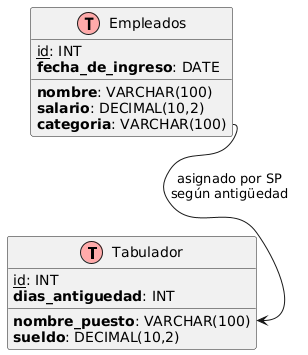
\includegraphics[width=0.7\textwidth]{DiagramaER.png}
\end{center}

\section*{Procedimiento en código}

\subsection*{Creación de la base de datos y tablas}

\begin{lstlisting}[language=SQL]
CREATE DATABASE EMPRESA;
USE EMPRESA;

CREATE TABLE Empleados (
  id INT AUTO_INCREMENT PRIMARY KEY,
  nombre VARCHAR(100),
  fecha_de_ingreso DATE,
  salario DECIMAL(10,2),
  categoria VARCHAR(100)
);

CREATE TABLE Tabulador (
  id INT AUTO_INCREMENT PRIMARY KEY,
  nombre_puesto VARCHAR(100),
  sueldo DECIMAL(10,2),
  dias_antiguedad INT
);
\end{lstlisting}

\subsection*{Inserción de datos en el tabulador}

\begin{lstlisting}[language=SQL]
INSERT INTO Tabulador (nombre_puesto, sueldo, dias_antiguedad) VALUES 
('Trainee', 1000.00, 1),
('Dev Junior', 5000.00, 12),
('Dev Senior', 10000.00, 20);
\end{lstlisting}

\subsection*{Inserción de empleados de prueba}

\begin{lstlisting}[language=SQL]
INSERT INTO Empleados (nombre, fecha_de_ingreso, salario, categoria) VALUES
('Ana Torres',      CURDATE() - INTERVAL 1 DAY,   0.00, 'Por definir'),
('Luis G\'omez',      CURDATE() - INTERVAL 2 DAY,   0.00, 'Por definir'),
('Mar\'ia L\'opez',     CURDATE() - INTERVAL 3 DAY,   0.00, 'Por definir'),
('Carlos M\'endez',   CURDATE() - INTERVAL 5 DAY,   0.00, 'Por definir'),
('Julia R\'ios',      CURDATE() - INTERVAL 7 DAY,   0.00, 'Por definir'),
('Pedro Jimenez',   CURDATE() - INTERVAL 9 DAY,   0.00, 'Por definir'),
('Luc\'ia Castro',    CURDATE() - INTERVAL 10 DAY,  0.00, 'Por definir'),
('Miguel Serrano',  CURDATE() - INTERVAL 12 DAY,  0.00, 'Por definir'),
('Elena Vargas',    CURDATE() - INTERVAL 15 DAY,  0.00, 'Por definir'),
('Jorge Pe\~na',      CURDATE() - INTERVAL 18 DAY,  0.00, 'Por definir'),
('Valeria Cruz',    CURDATE() - INTERVAL 20 DAY,  0.00, 'Por definir'),
('Santiago Ruiz',   CURDATE() - INTERVAL 22 DAY,  0.00, 'Por definir'),
('Gabriela Mora',   CURDATE() - INTERVAL 25 DAY,  0.00, 'Por definir'),
('Hugo Castillo',   CURDATE() - INTERVAL 27 DAY,  0.00, 'Por definir'),
('Laura Fern\'andez', CURDATE() - INTERVAL 30 DAY,  0.00, 'Por definir');
\end{lstlisting}

Se inicializa a todos los empleados con salario 0.00 y categoría ``Por definir'' para verificar claramente los cambios después de aplicar el procedimiento.

\subsection*{Creación del Stored Procedure}

\begin{lstlisting}[language=SQL]
DELIMITER $$

CREATE PROCEDURE ActualizarSalarioYCategoria()
BEGIN
  UPDATE Empleados e
  JOIN (
    SELECT 
      e.id,
      t.nombre_puesto,
      t.sueldo
    FROM Empleados e
    JOIN Tabulador t
      ON DATEDIFF(CURDATE(), e.fecha_de_ingreso) >= t.dias_antiguedad
    WHERE
      t.dias_antiguedad = (
         SELECT MAX(t2.dias_antiguedad)
         FROM Tabulador t2
         WHERE DATEDIFF(CURDATE(), e.fecha_de_ingreso) >= t2.dias_antiguedad
       )
  ) AS sub
  ON e.id = sub.id
  SET 
    e.salario = sub.sueldo,
    e.categoria = sub.nombre_puesto;
END$$

DELIMITER ;
\end{lstlisting}

Este procedimiento compara la antigüedad de cada empleado con los requisitos definidos en el `Tabulador`, y actualiza su salario y categoría al más alto que le corresponda.

\subsection*{Creación de un evento programado diario}

\begin{lstlisting}[language=SQL]
CREATE EVENT IF NOT EXISTS evento_actualizar_salarios_y_categorias
ON SCHEDULE EVERY 1 DAY
STARTS CURRENT_DATE + INTERVAL 2 HOUR
DO
  CALL ActualizarSalarioYCategoria();
\end{lstlisting}

El evento anterior asegura que la actualización se ejecute automáticamente todos los días a las 2:00 a.m.

\section*{Fase de pruebas}

\subsection*{Tabla antes de ejecutar el procedimiento}
\begin{center}
  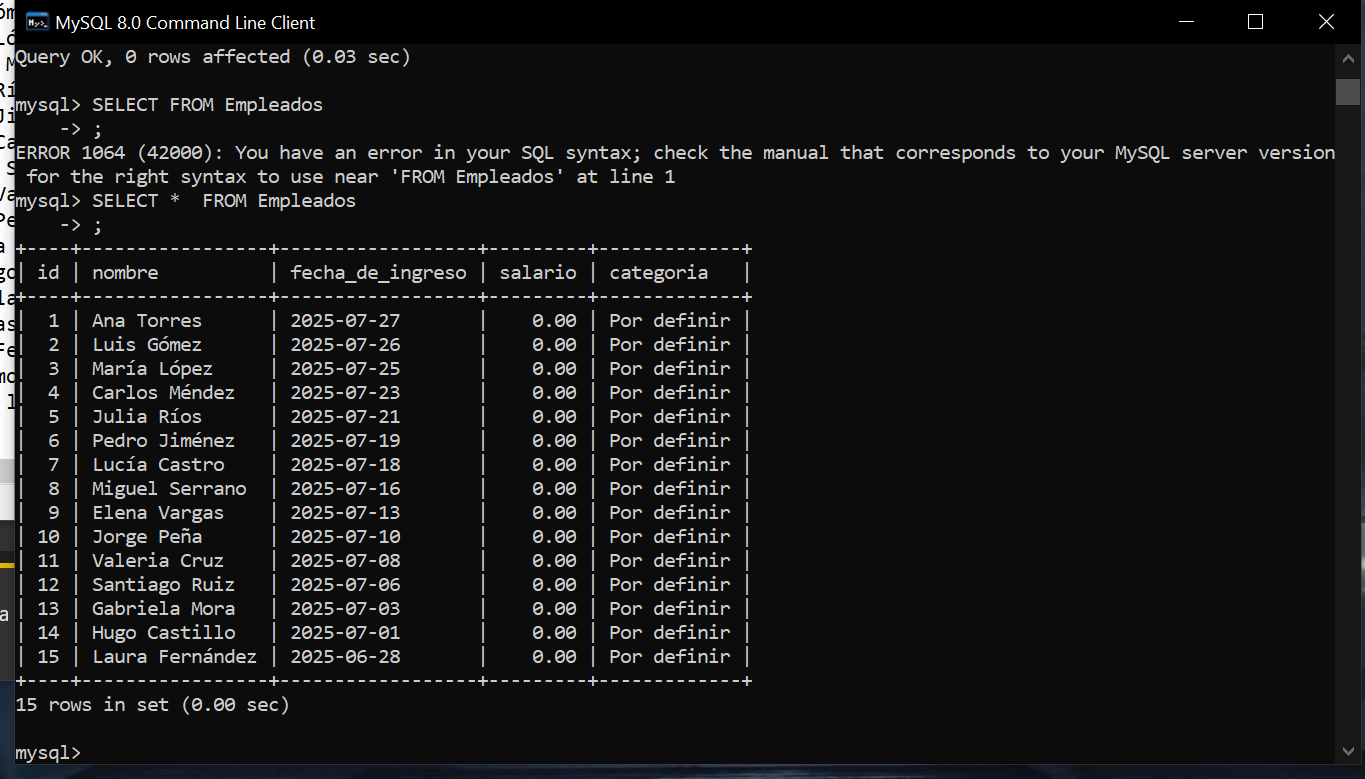
\includegraphics[width=0.85\textwidth]{EmpleadosInicial.png}
\end{center}

\subsection*{Evidencia de creación y ejecución del procedimiento}
\begin{center}
  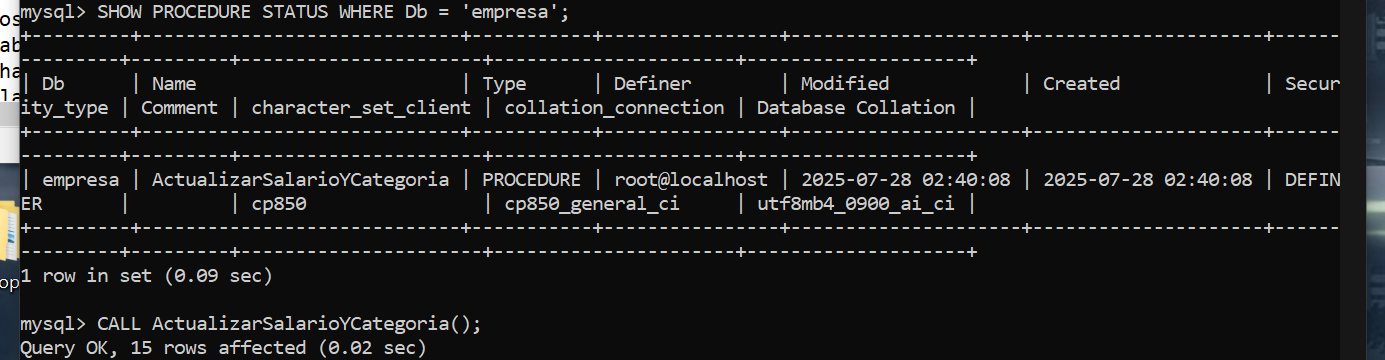
\includegraphics[width=0.85\textwidth]{StoreProcedure.png}
\end{center}

\subsection*{Resultados después de aplicar el procedimiento}
\begin{center}
  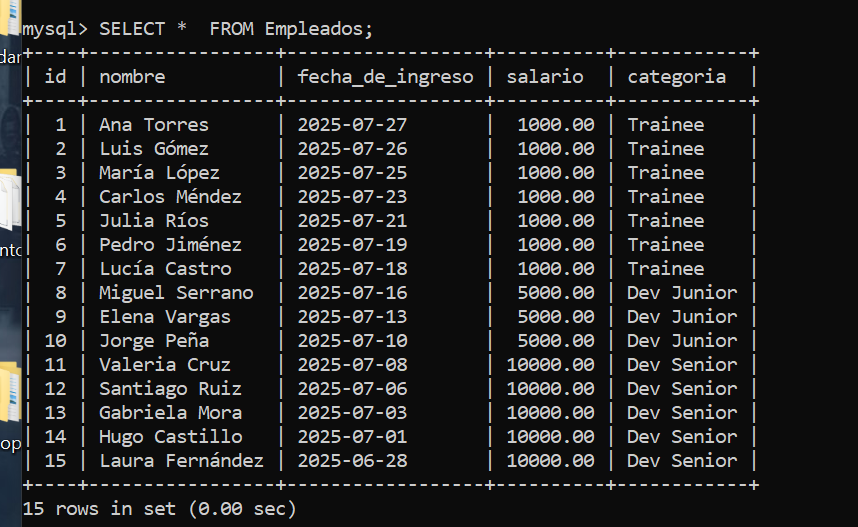
\includegraphics[width=0.85\textwidth]{EmpleadosPrueba.png}
\end{center}

\end{document}
